%!TEX root = ./main.tex
\begin{frame}[fragile]{Conclusion}
    
    \pause

    \begin{itemize}
        \item <2-> Approach has been implemented in a Java prototype
    \end{itemize}

    \pause

    \begin{figure}
        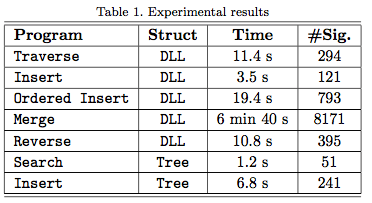
\includegraphics[scale=0.5]{images/ResultTable.png}
        \\ \tiny{Prototype Results \cite{abdulla2013monotonic}}
    \end{figure}
\end{frame}

\begin{frame}[fragile]{Conclusion}
    
    \pause

    \begin{itemize}
        \item <2-> Relatively simple method
        \item <3-> Very generic approach
        \item <4-> Successfully implemented
    \end{itemize}

\end{frame}

\begin{frame}[fragile]{Conclusion}
    
    Any questions?

\end{frame}